\documentclass{article}

% \usepackage[UTF8, scheme = plain]{ctex}
\usepackage{fancyhdr}   % 页眉, 页脚, 页码设置
\usepackage{extramarks} % 
\usepackage{amsmath}    % 公式
% \usepackage{amsthm}     % 数学定理之类的,提供了 proof 等包 
% \usepackage{amsfonts}   % 数学字体
\usepackage{tikz}       % 绘图宏包 
% \usepackage[plain]{algorithm} % 制作算法图,伪代码
% \usepackage{algpseudocode}    % 伪代码
\usepackage{color}      % 颜色 (包括文字颜色等)
% \usepackage{listings}   % 代码, 使用xelatex
\usepackage{fontspec}   % 修改字体
\usepackage{float}      % 固定图片位置
\usepackage{indentfirst}      % 首行缩进

\setlength{\parindent}{2em}  %% 首行缩进
\setlength{\parskip}{1em} %% 设置段落间距
\linespread{1.1}    %% line spacing
\definecolor{ustcblue}{cmyk}{1,0.8,0,0}  %% ustc logo 颜色
\setmainfont{Times New Roman} %% 设置字体

% \newfontfamily\menlo{Menlo}
% % \newfontfamily\menlo{Consolas}
% \lstset{
%     columns=fixed,       
%     numbers=left,                                        % 在左侧显示行号
%     numberstyle=\tiny\color{gray},                       % 设定行号格式
%     frame=none,                                          % 不显示背景边框
%     backgroundcolor=\color[RGB]{245,245,244},            % 设定背景颜色
%     keywordstyle=\color[RGB]{40,40,255},                 % 设定关键字颜色
%     numberstyle=\footnotesize\color{darkgray},           
%     commentstyle=\it\color[RGB]{0,96,96},                % 设置代码注释的格式
%     stringstyle=\rmfamily\slshape\color[RGB]{128,0,0},   % 设置字符串格式
%     showstringspaces=true,                              % 不显示字符串中的空格
%     numberstyle=\small\menlo,
%     basicstyle=\small\menlo,
%     breaklines=true,
% }

%
% Basic Document Settings
%
%%% page layout
\topmargin=-0.45in
\evensidemargin=0in
\oddsidemargin=0in
\textwidth=6.5in
\textheight=9.0in
\headsep=0.25in

\pagestyle{fancy}
\lhead{\hmwkAuthorName}
\chead{\hmwkClass\ (\hmwkClassInstructor): \hmwkTitle}
\rhead{}
\lfoot{}
\cfoot{\thepage}

\renewcommand\headrulewidth{0.4pt}
\renewcommand\footrulewidth{0.4pt}

%
% Create Problem Sections
%

\newcommand{\enterProblemHeader}[1]{
    \nobreak\extramarks{}{Problem \arabic{#1} continued on next page\ldots}\nobreak{}
    \nobreak\extramarks{Problem \arabic{#1} (continued)}{Problem \arabic{#1} continued on next page\ldots}\nobreak{}
}

\newcommand{\exitProblemHeader}[1]{
    \nobreak\extramarks{Problem \arabic{#1} (continued)}{Problem \arabic{#1} continued on next page\ldots}\nobreak{}
    \stepcounter{#1}
    \nobreak\extramarks{Problem \arabic{#1}}{}\nobreak{}
}

\setcounter{secnumdepth}{0}
\newcounter{partCounter}
\newcounter{homeworkProblemCounter}
\setcounter{homeworkProblemCounter}{1}
\nobreak\extramarks{Problem \arabic{homeworkProblemCounter}}{}\nobreak{}

%
% Homework Problem Environment
%
% This environment takes an optional argument. When given, it will adjust the
% problem counter. This is useful for when the problems given for your
% assignment aren't sequential. See the last 3 problems of this template for an
% example.
%
\newenvironment{homeworkProblem}[1][-1]{
    \ifnum#1>0
        \setcounter{homeworkProblemCounter}{#1}
    \fi
    \subsection{Exercise \arabic{homeworkProblemCounter}}
    \setcounter{partCounter}{1}
    \enterProblemHeader{homeworkProblemCounter}
}{
    \exitProblemHeader{homeworkProblemCounter}
}


\newcommand{\hmwkTitle}{Homework\ \#3}
\newcommand{\hmwkDueDate}{\today}
\newcommand{\hmwkClass}{Geodynamics}
\newcommand{\hmwkClassInstructor}{Professor W. Len}
\newcommand{\hmwkAuthorName}{\textbf{Jintao Li}}
\newcommand{\hmwkAuthorID}{\textbf{SA20007037}}
\newcommand{\hmwkAuthoremail}{\textbf{E-mail: lijintao@mail.ustc.edu.cn}}


\renewcommand{\part}[1]{\textbf{ \\ (\alph{partCounter})  }\stepcounter{partCounter} }

% Alias for the Solution section header
\newcommand{\solution}{\textbf{\large \\ Solution: \\}}

%%%%
\newcommand{\mb}[1]{\mathbf{#1}}



\begin{document}

\begin{titlepage}
\begin{center}

\textcolor{ustcblue}{
\includegraphics[width=0.4\textwidth]{../../inversion/ustc_logo_fig.pdf} \\ [1cm]}
% Title
{ \Huge \bfseries \hmwkClass\ \hmwkTitle}\\[1cm]

\large \textbf{\hmwkClassInstructor} \\ [5cm]

\large \hmwkAuthorName \\ [0.25cm]
\large \hmwkAuthorID \\ [0.25cm]
\large \hmwkAuthoremail
\vfill
% Bottom of the page
{\large \hmwkDueDate}

\end{center}
\end{titlepage}

\begin{center}
\section{Chapter 3: Elasticity and Flexure}
\end{center}


\begin{homeworkProblem}
The effect of large scale volcanic eruption on the crustal flexture.
\begin{figure}[H]
    \centering
    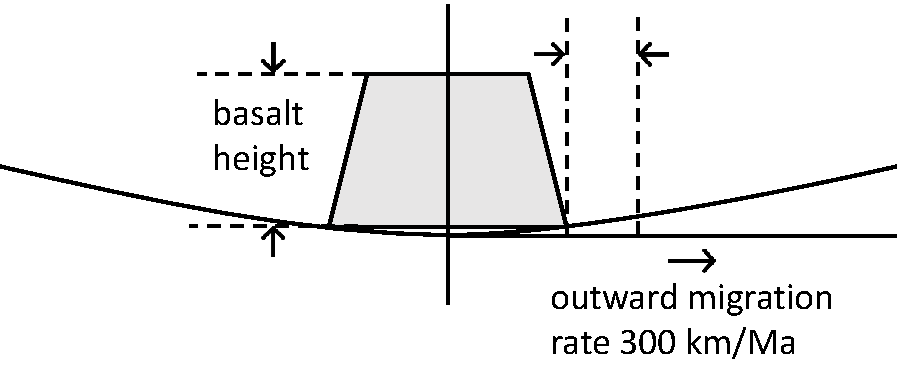
\includegraphics[width=6in, keepaspectratio]{fig01.pdf}
    \label{fig:fig01}
\end{figure}

Suppose volcanic eruption lasts for 2 $Ma$, forming
basalts accumulation with a height of 2 $km$. The
cross-section shape of the basalts are trapezoid, the
upper boundary of the trapezoid is 0.8 of the bottom
boundary. Basalts spread from the center at a speed of
300 $km/Ma$.
Some parameters: Young’s modulus 70 $GPa$, poisson's ratio 0.25, 
density of the basalts 2700 $kg/m^3$, crust density
2900 $kg/m^3$, elastic thickness of the crust 50 $km$.

Solve for the time variation of surface topography at
x=150, 300 and 450 $km$ from the eruption center.
Discuss the effects of different elastic thickness on the
results.


\solution

Refering to Brotchie's paper \textit{On Crustal Flexure}, the differential 
equation for deflection can be represented as:
\begin{equation}
    D \nabla^{4} w+\left(E T / R^{2}\right) w+\gamma w=q .
\end{equation}
And rewriting the formula in plane polar coordinate and the spherical coordinates of
the shell, it can be:
\begin{equation}
    \nabla^{4} w+\left(1 / l^{4}\right) w=q / D ,
    \label{eq:02}
\end{equation}
in which $l^{4} \equiv D /\left[\left(E T / R^{2}\right)+\gamma\right]$, $\omega$ 
is the radial displacementof the shell undernormalloadingof intensityq, D is
the flexural stiffness of the shell cross section 
$\equiv \left[E T^{3} / 12\left(1-v^{2}\right)\right]$, $T$ is the thickness of the
shell, $E$ is itsmodulusof elasticity, $\upsilon$ is Poisson's ratio for the 
shellmaterial, $R$ is the radius of its middle surface, $\gamma$ is the density 
of the enclosed liquid. 

We consider this the volcanic loading as \textit{variable loading}. 
And the deflections of crust for a volcanic eruption of variable thickness 
are found by superposition using uniform thickness solution. The variable 
thickness may be approximated by a stepped distribution. The sheet may then 
be considered to be composed of uniform layers of depth $h$ and radius $a_n$, 
and we choose step size $h = 5 m$. 

As to uniform loading, solving
the equation~\ref{eq:02}, we can obtain the solution:
\begin{equation}
    w_{i}=\frac{\gamma_{volcanic} h}{\gamma^{\prime}}
    \left(a \operatorname{ker}^{\prime} a \operatorname{ber} x - a 
    \operatorname{kei}^{\prime} a \operatorname{bei} x+1\right) ,
\end{equation}
and, outside the volcanic eruption, deflection $omega_0$ is:
\begin{equation}
    w_{0}=\frac{\gamma_{volcanic} h}{\gamma^{\prime}}
    (a \operatorname {ber}^{\prime} a \operatorname{ker} x
    - a \operatorname{bei}^{\prime} a \operatorname{kei} x) ,
\end{equation}
in which $h$ is uniform depth, $\gamma_{volcanic}$ is the density of basalts,
$\gamma$ is the density of mantle, and $\gamma^{\prime} = \gamma + ET/R^2$.

\end{homeworkProblem}

\end{document}
